\documentclass{article}
\usepackage[T1]{fontenc}
\usepackage{lmodern}
\usepackage{graphicx}
\usepackage{amsmath,amssymb}
\usepackage[a4paper,margin=2cm]{geometry}
\usepackage[absolute,overlay]{textpos}
\setlength{\TPHorizModule}{1mm}
\setlength{\TPVertModule}{1mm}
\usepackage[indonesian]{babel}
\usepackage{hyperref}
\setlength{\emergencystretch}{2em}
% unit: Halaman 29

\begin{document}

% === Halaman 29 (llm) ===

% (tidak ada teks dari model)

% deskripsi: Diagram alur proses steganografi yang menunjukkan proses embedding pada sisi pengirim (sender) menggunakan cover-object dan stego-key, pengiriman stego-object melalui jaringan (network), dan proses ekstraksi pada sisi penerima (receiver) untuk mendapatkan pesan yang disembunyikan (extracted message).
% bbox normalisasi: [0.0700, 0.2300, 0.9170, 0.8100]
\begin{textblock*}{177.87mm}(14.70mm,68.31mm)
\noindent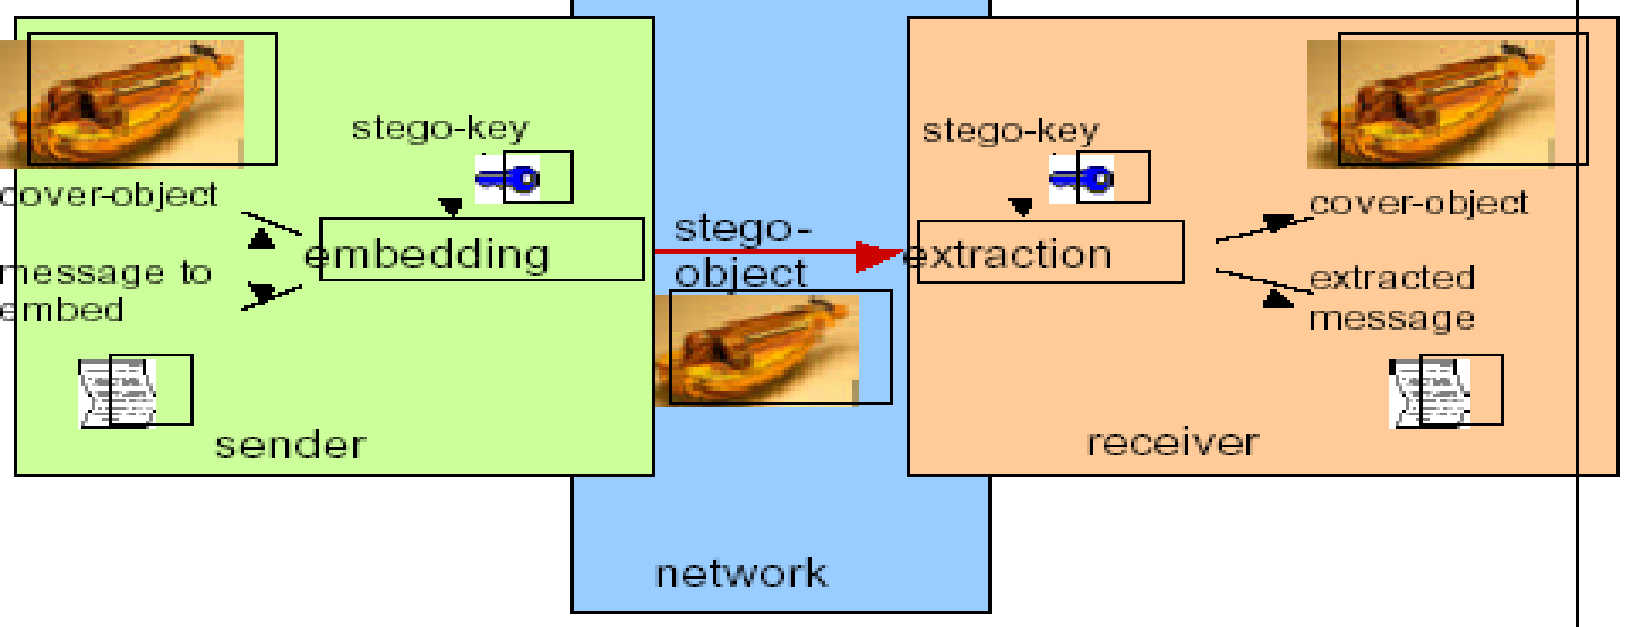
\includegraphics[width=177.87mm,height=172.26mm]{../../images/llm/page_029_img_01.png}%
\end{textblock*}

\end{document}
